\input{../../preamble2.tex}
\begin{document}
\begin{center}
	\Huge\textbf{Математический анализ}
\end{center}
\tableofcontents
\newpage
\begin{center}
\large{\textbf{Модуль №1} \\
\textit{Элементарные функции и пределы}}
\end{center}
\input{Основы математического анализа.tex}
\newpage
\zerocounter
\input{Числовая последовательность.tex}
\newpage
\zerocounter
\input{Предел функции.tex}
\newpage
\zerocounter
\input{бмф. Арифметические операции.tex}
\newpage
\zerocounter
\input{Предел функции. бмф ббф.tex}
\newpage
\zerocounter
\input{Непрерывность функции. Точки разрыва.tex}
\newpage
\zerocounter
\begin{center}
\large{\textbf{Модуль №2} \\
\textit{Дифференциальное исчисление функции одной переменной}}
\end{center}
\input{Производная функции.tex}
\newpage
\zerocounter
\input{Дифференциал функции.tex}
\zerocounter
\newpage
input{Основные теоремы дифференциального исчисления.tex}
\newpage
\zerocounter
\input{Раскрытие неопределённостей.tex}
\zerocounter
\newpage
\input{Формула Тейлора.tex}
\zerocounter
\newpage
%%%%%%%%%%%%%%%%%%%%

\section{Вертикальные, наклонные, горизонтальные асимптоты}
\begin{definition}
	\textbf{Асимптотой} графика функции $y=f(x)$ называется прямая, расстояние до которой от точки, лежащей на графике, стремится к нулю при удалении от начала координат.
\end{definition} \vspace{-\topsep}
\begin{figure}[h]
	\centering
	\begin{tikzpicture}[scale=1, thick]
		\tkzInit[xmin=-0.5, xmax=7, ymin=-1.5, ymax=1.5]
		\tkzDrawX \tkzDrawY
		\draw[domain=0:7,smooth,variable=\x, samples=200, very thick] plot ({\x},{1.5*exp(-0.3*\x)*sin(deg(5*\x))});
		\node at (5, 1.5) {Затухающие колебания};
	\end{tikzpicture}
\end{figure} \vspace{-\topsep}
\begin{center}
\begin{tikzcd}[row sep=12pt, column sep=0pt, scale cd = 1]
 & \text{Асимптоты}\arrow[ld]\arrow[d]\arrow[rd] & \\
\text{вертикальные} & \text{наклонные} & \text{горизонтальные} 
\end{tikzcd}
\end{center}	
\begin{definition}
	Прямая $x=a$ называется \textbf{вертикальной асимптотой} графика функции $y=f(x)$, если хотя бы один из пределов $\lim\limits_{x \to a+} f(x)$, $\lim\limits_{x \to a-} f(x)$ равен $\infty$.
\end{definition}
\subsection*{Примеры}
\begin{eg}
	\begin{flalign*}
		& y = \frac{1}{x-a}\hspace{5cm} &\\[1ex]
		& \begin{aligned} 
			&\lim\limits_{x \to a+} \frac{1}{x-1} = \frac{1}{0+} = +\infty\\
			&\lim\limits_{x \to a-} \frac{1}{x-a} = \frac{1}{0-} = -\infty  
		\end{aligned}\ \Rightarrow\ x=a \text{ --- }
		\begin{aligned} 
			&\text{вертикальная} \\
			&\text{асимптота} &
		\end{aligned}
	\end{flalign*} \vspace{-13\topsep}
	\begin{flushright}
		\begin{tikzpicture}[scale=0.7, thick]
			\tkzInit[xmin=-3, xmax=4, ymin=-3, ymax=4]
			\tkzDrawX \tkzDrawY
			\draw[very thick] (-3, -0.2) .. controls (0.25, -0.25) and (0.75, -0.25).. (0.9, -3) ;
			\draw[very thick] (1.1, 4) .. controls (1.25, 1) and (1.75, 0.25) .. (4, 0.2);
			\draw[dashed] (1, -3) -- (1, 4);
			\node at (3, 3) {$y=\dfrac{1}{x-a}$};
			\node[above left] at (0, 0) {$0$};
			\node[below left] at (1, 0) {$a$};
		\end{tikzpicture}
	\end{flushright} 
\end{eg}
\begin{eg}
	\begin{flalign*}
		& y = \ln x &\\
		& D_y\colon (0; +\infty) &\\
		& \lim\limits_{x \to 0+} \ln x = (-\infty) &
	\end{flalign*}
	\vspace{-10\topsep}
	\begin{flushright}
		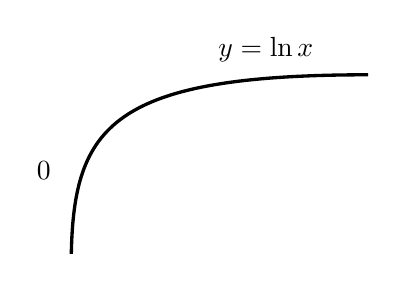
\begin{tikzpicture}[scale=0.65, thick]
			\tkzInit[xmin=-1, xmax=6, ymin=-2, ymax=3]
			\tkzDrawX \tkzDrawY
			\draw[very thick] (0.2, -2) .. controls (0.25, 0.5) and (1, 1.5) .. (6, 1.5) ;
			\node at (4, 2) {$y=\ln x$};
			\node[below left] at (0, 0) {$0$};
		\end{tikzpicture}
	\end{flushright} 
\end{eg}
\textbf{Вывод}:
Вертикальные асимптоты ищем среди точек разрыва функции и граничных точек.
\subsection{Наклонные асимптоты}
\begin{definition}
	Прямая $y=kx+b$ называется \textbf{наклонной асимптотой} графика функции $y=f(x)$ при $x \to \pm \infty$, если функция $f(x) = kx+b + \alpha(x)$, где $\alpha(x)$ --- б.м.ф. при $x\to \pm \infty$.
\end{definition}
\begin{theorem}[Необходимое и достаточное условие существования наклонных асимптот]
	График функции $y=f(x)$ имеет при $x\to \pm \infty$ наклонную асимптоту тогда и только тогда, когда существуют два конечных передела:
	\begin{gather*}
		\left\{ \begin{aligned}
			& \lim\limits_{x \to \pm \infty} \frac{f(x)}{x} = k \\
			& \lim\limits_{x \to \pm \infty} \left(f(x) - k\cdot x\right) = b
		\end{aligned} \tag{$*$} \right.
	\end{gather*} 
\end{theorem}
\begin{proof}[][Необходимость]
	\textbf{Дано}: $y=kx+b$ --- наклонная асимптота\\
	\textbf{Доказать}: $\exists$ конечные пределы $(*)$\\
	По условию $kx+b$ наклонная асимптота $\Rightarrow$ по определению наклонной асимптоты: $f(x) = kx + b + \alpha(x)$, где $\alpha(x)$ -- б.м.ф. при $x \to \pm \infty$.\\
	Рассмотрим:
	\begin{flalign*}
		\lim\limits_{x \to \pm \infty} \frac{f(x)}{x} = \lim\limits_{x \to \pm \infty} \frac{kx + b + \alpha(x)}{x} & = \lim\limits_{x \to \pm \infty} \left(k + b\cdot \frac{1}{x} + \frac{1}{x}\cdot \alpha(x)\right) = &\\
		& = k + b\cdot \lim\limits_{x \to \pm \infty} \frac{1}{x} + \lim\limits_{x  \to \pm \infty} \frac{1}{x}\cdot \alpha(x) = k + b\cdot 0 + 0 = k &
	\end{flalign*}
	Рассмотрим выражение:
	\begin{gather*}
		f(x) - k\cdot x = \cancel{kx} + b + \alpha(x) - \cancel{kx} = b + \alpha(x)
	\end{gather*}
	Вычислим:
	\begin{flalign*}
		& \lim\limits_{x \to \pm \infty} \big(f(x) - k\cdot x\big) = \lim\limits_{x \to \pm \infty} \big(b + \alpha(x)\big) = b + \lim\limits_{x \to \pm \infty} \alpha(x) = b + 0 = b
	\end{flalign*}
\end{proof}
\begin{proof}[][Достаточность]
	\textbf{Дано}: $\exists$ конечные пределы $(*)$\\
	\textbf{Доказать}: $y=kx+b$ --- наклонная асимптота\\[1ex]
	$\exists$ конечный предел: $\lim\limits_{x \to \pm \infty} (f(x) - kx) = b$\\
	По теореме \textit{о связи функции, её предела и б.м.ф.} (\textbf{С.\pageref{О связи функции, её предела и б.м.ф.}, Т.\ref{О связи функции, её предела и б.м.ф.}}) $\Rightarrow$\\
	$\Rightarrow\ f(x) - kx = b + \alpha(x)$, где $\alpha(x)$ -- б.м.ф. при $x \to \pm \infty$.\\
	Выразим $f(x) = kx + b + \alpha(x)$, где $\alpha(x)$ -- б.м.ф. при $x \to \pm \infty$.\\
	По определению наклонной асимптоты $\Rightarrow\ y = kx + b$ --- наклонная асимптота графика функции $y=f(x)$.
\end{proof}
\newpage
\subsection{Горизонтальные асимптоты}
\begin{definition}
	Прямая $y=b$ называется \textbf{горизонтальной асимптотой} функции $y=f(x)$, если $\lim\limits_{x \to \pm \infty} f(x) = b$.
\end{definition}
\begin{corollary*}
	Горизонтальные асимптоты являются частным случаем наклонных асимптот при $k=0$.
\end{corollary*}
\zerocounter
\section{Исследование функции $y = f(x)$ по первой производной}
\begin{definition}
	Функция $y=f(x)$, определённая на $(a;b)$, \textbf{возрастает} (\textbf{убывает}) на этом интервале, если: \[ \forall\ x_1, x_2 \in (a;b)\colon x_2 > x_1\ \Rightarrow\ f(x_2) > f(x_1)\quad \Big(f(x_2) < f(x_1)\Big) \]
\end{definition}
\begin{definition}
	Функция $y=f(x)$, определённая на $(a;b)$, \textbf{не убывает} (\textbf{не возрастает}) на этом интервале, если:
	\[ \forall\ x_1, x_2 \in (a;b)\colon x_2 > x_1\ \Rightarrow\ f(x_2) \ge f(x_1)\quad \Big(f(x_2) \le f(x_1)\Big) \]
\end{definition}
\begin{definition}
	Невозрастающая, неубывающая, возрастающая, убывающая функции называются \textbf{монотонными} функциями.
\end{definition}
\begin{definition}
	Возрастающая и убывающая функции называются \textbf{строго монотонными} функциями.
\end{definition}
\begin{theorem}[Необходимое и достаточное условие невозрастания | неубывания дифференцируеммой функции]
	Дифференцируемая на интервале $(a;b)$ функция $y=f(x)$ не возрастает (не убывает) на этом интервале тогда и только тогда, когда:
	\[ f'(x) \le 0\ \Big(f'(x) \ge 0\Big)\quad \forall\ x \in (a;b) \]
\end{theorem}
%%%%%%%%%%%%%%%%%%%%
\end{document}